\subsection{Analytical Solution}\label{analyticalSolution}

\begin{figure}[ht]
\centering\fbox{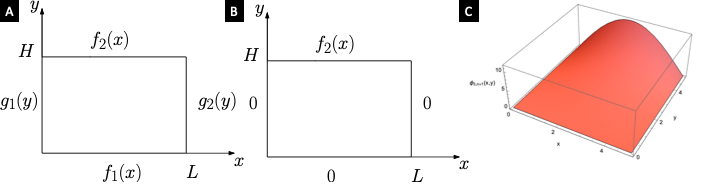
\includegraphics[height=1.5in,width=4.5in]{figures/figures2/00_analytical_pde.png}}
\caption{\textbf{(A)} The four boundaries of $\psi \left(x,y \right)$ are defined in terms of the $x$ and $y$ axis. \textbf{(B)} The one non-zero boundary condition and three zero boundary conditions for the $\varphi_3\left(x,y\right)$ solution component of $\varphi \left(x,y \right)$. \textbf{(C)} Plot of $\psi_{3,n}\left(x,y\right)$ with $n=1$, $L=5$ and $H=5$ with the continuous solution shown in the z axis.}
\label{fig:pdeBoundary}
\end{figure}

Laplace's equation is a second-order partial differential equation which produces, as a solution, harmonic functions that accurately describe the behavior of electric, gravitational and fluid potentials.  It has no time dependence, only a spatial dependence, and is often written as  

\begin{equation}\label{}
\nabla^2 \varphi = 0
\end{equation}

where \(\nabla^2\) is the Laplace operator and \(\varphi\) is a scalar function.

For the purpose of simplicity, we will only discuss spatial variables $x$ and $y$, which allows Laplace's equation to be rewritten as

\begin{equation}\label{eq:Laplace2D}
\frac{\partial^2 \varphi}{\partial x^2} + \frac{\partial^2 \varphi}{\partial y^2} = 0
\end{equation}

Following the derivation in section \ref{section:pdeDerivation} \cite{vrscay2010amath} results in the product solutions yielded by the separation of variables method up to a constant.

\begin{equation}\label{eq:sovSol_a}
\begin{aligned} 
\varphi _ { 3 , n } \left( x , y \right) & 
= \sin \left( \frac { n \pi x } { L } \right) \sinh \left(\frac { n \pi y } { L } \right)
& \text{for } n=1,2,3,\dots
\end{aligned}
\end{equation}

\subsection{Physical Units}\label{physicalUnits}
Why is necessary to discuss the physical interpretation of the purely mathematical solution of the Laplacian partial differential equation? To better understand the source of inaccuracies that deviate from the analytical solution derived in Section \ref{analyticalSolution} caused by discretization and the implementation of different analog algorithms built on physical hardware we must first address the inequality of units associated with the generated solutions. The analytical solution is purely mathematical and therefor unitless. The digitally generated discretized numerical solution outputs heat map in Kelvin [\SI{}{\kelvin}]. The electrical analog algorithm mesh can sample solutions either in Volts [\SI{}{\volt}] or current [\SI{}{\ampere}]. Photoinc ROC outputs solutions in Optical Intensity [\SI{}{\watt \meter^{-2}}]. Metatronic ROC outputs solutions in Electric Displacement Current Density $J_D$ [\SI{}{\ampere \meter^{-2}}].
\par Initially we have been normalizing all our solutions between zero and one. However to determine true equivalence in the future we can potentially add physics to our analytical solution and generate a solution for a temperature distribution in Kelvin [\SI{}{\kelvin}]. By mapping electrical, photonic ROC, and metatronic ROC to an equivalent temperature distribution in Kelvin, we can remove unit mismatch as a source of inaccuracy.